\section{\scshape Introduction}
\subsection{OSSIA}
\begin{frame}{OSSIA}
	{\large Open Scenario System for Interactive Applications}
	
	Utilise les acquis de plusieurs années de développement au \textsc{LaBRI} et au \textsc{SCRIME}; basé sur le projet \textsc{ANR Virage}.
	
	\vspace{1em}
	Aspect majeur : \emph{temps}.
	\begin{itemize}
		\itemar Est implémenté avec la notion de scénario et d'évènement.
		\itemar Interactivité du temps : temps souple, conditionnel et points d'interaction.
	\end{itemize}
	
	Aspect majeur : \emph{inter-opérabilité}.
	\begin{itemize}
		\itemar Est implémenté avec le protocole \textsc{Minuit}.
	\end{itemize}
	
	La notion de processus relie temps et inter-opérabilité. Ces relations sont précisées dans \cite{hogue2014ossia}.
\end{frame}

\begin{frame}{Exemple de scénario}
	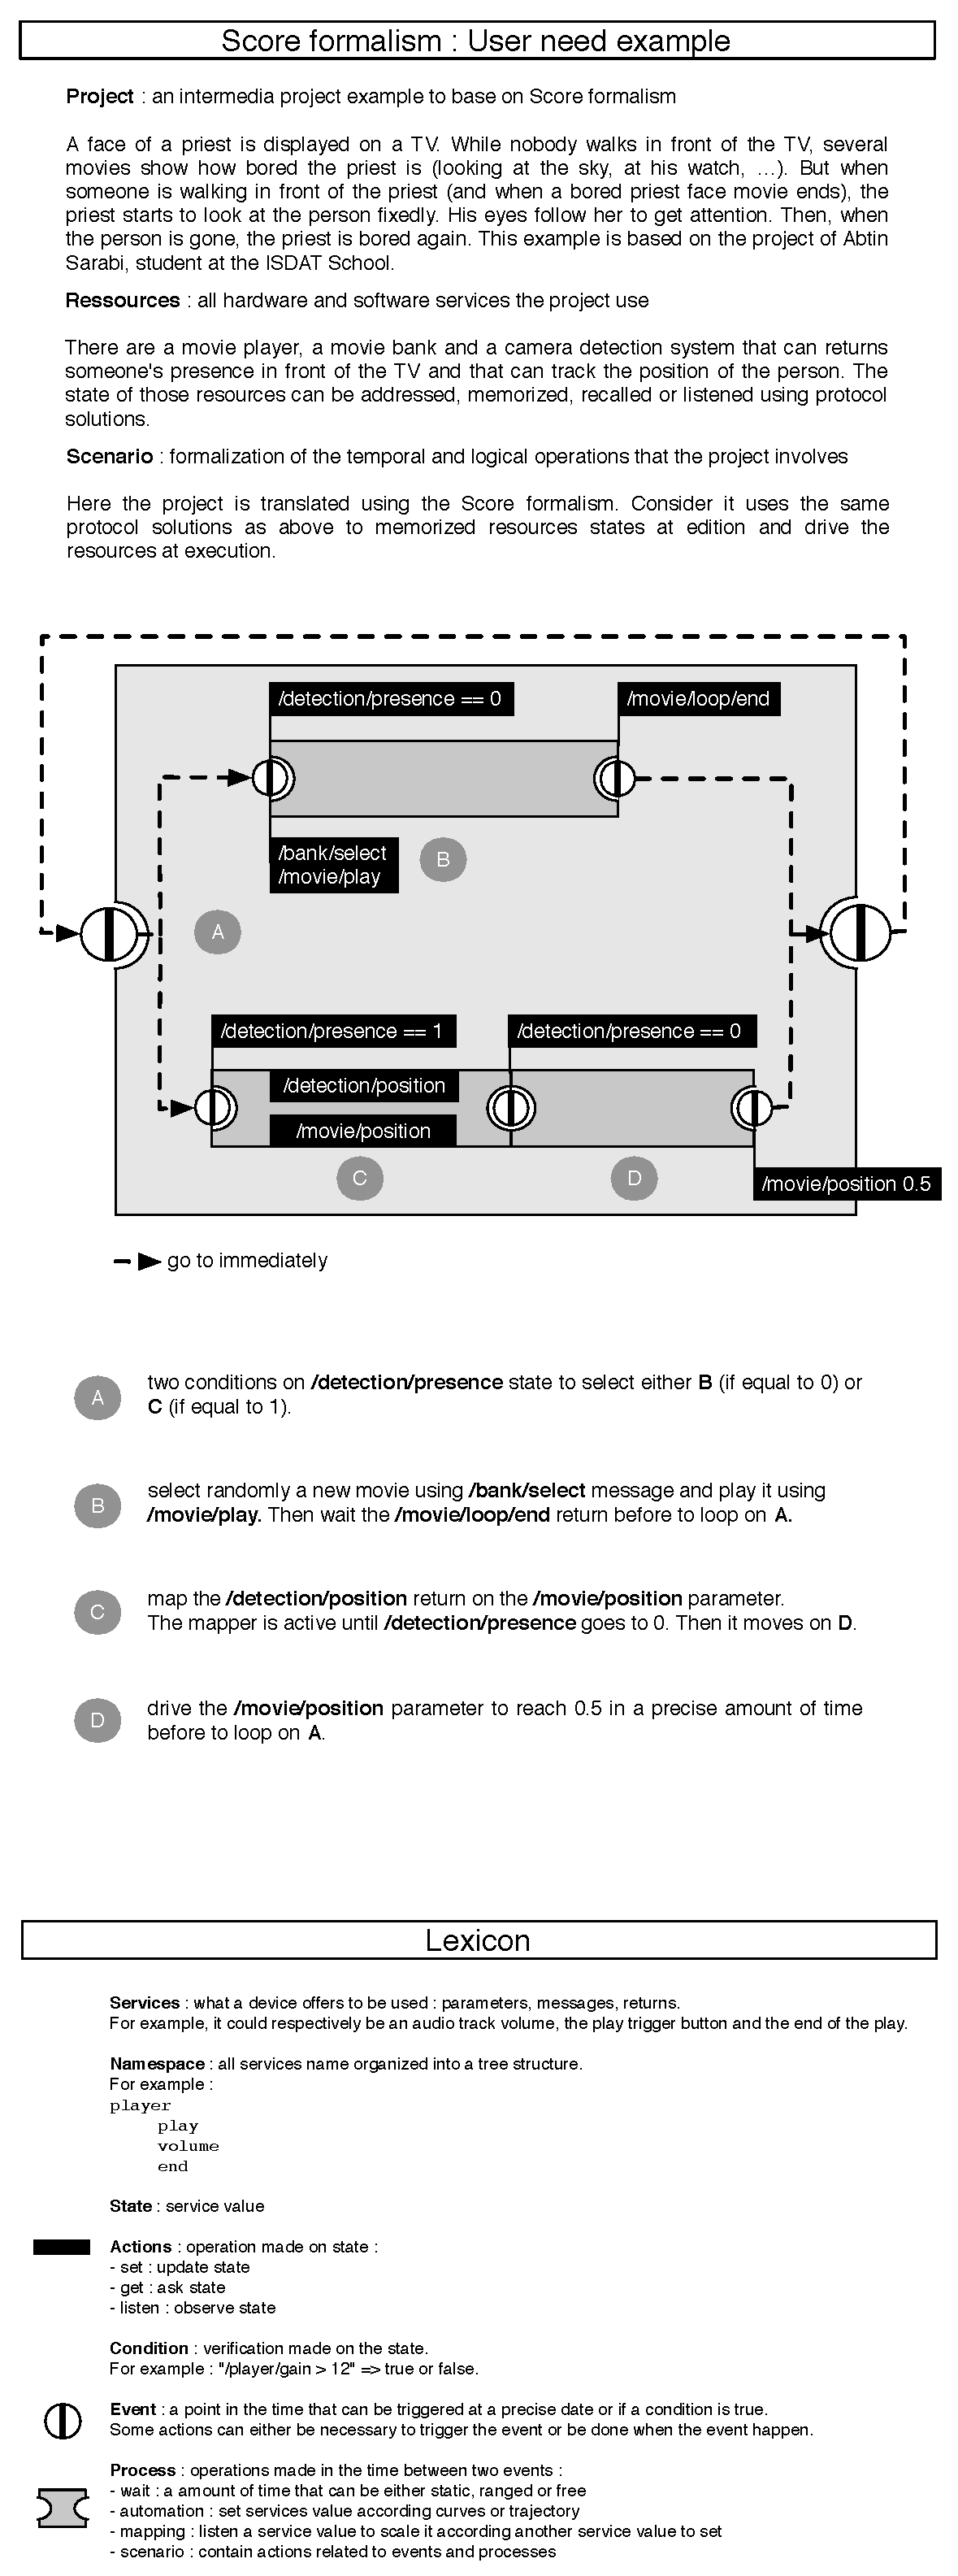
\includegraphics[scale=0.5,clip,trim=0cm 28cm 0cm 13cm]{../src/images/moineOSSIA.pdf}
\end{frame}

\subsection{Sujet}
\begin{frame}{Sujet du mémoire}
	{\large Répartition des réseaux de Petri dans i-score}
	
	Aspects principaux : 
	\begin{itemize}
		\item Réseaux de Petri $\rightarrow$ recherche d'existant et étude théorique.
		\item i-score $\rightarrow$ implémentation dans un logiciel existant.
	\end{itemize} 
	\vspace{1em}
	Aspects apparus par la suite : 
	\begin{itemize}
		\item Édition collaborative.
		\item Fonctionnement avec les concepts {OSSIA}.
		\item Fonctionnement dans un cadre plus général que celui du logiciel, et sur plate-formes embarquées.
		\item Problématique de synchronisation.
	\end{itemize}
\end{frame}